\chapter{Revisión del Mercado de Aplicaciones}
\label{chap:mercado}

Antes de abordar el desarrollo del emulador, resulta fundamental \textbf{analizar el panorama actual de aplicaciones similares disponibles en el mercado}. Este capítulo tiene como objetivo \textbf{estudiar y comparar distintas soluciones} existentes que permiten emular juegos de Game Boy en dispositivos Android, \textbf{identificando sus características, puntos fuertes y limitaciones}.
\\\\
La revisión se centra en emuladores reconocidos como My OldBoy! y GBCC, \textbf{prestando especial atención} a aspectos como el \textbf{rendimiento}, la \textbf{interfaz de usuario}, y las \textbf{opciones de configuración}.
\\\\
Este análisis no solo proporciona una visión general del estado de la tecnología en este ámbito, sino que también permite \textbf{identificar oportunidades de mejora} y justificar las decisiones de diseño adoptadas en el presente proyecto.

\section{Referencias}
En esta sección se encuentran aquellas aplicaciones que, tras una revisión de los mismos, se cree que han sido de utilidad por su parecido a la hora de desarrollar este proyecto:

\subsubsection{My OldBoy!}

\textbf{My OldBoy!} es un emulador de Game Boy y Game Boy Color \textbf{diseñado específicamente para dispositivos Android}, que destaca por su precisión en la emulación de casi todos los aspectos del hardware original. Además de simular las consolas, soporta características especiales como el uso del cable link, la vibración y el sensor de inclinación.
\\\\
El emulador es \textbf{altamente valorado por su interfaz intuitiva y las múltiples opciones de personalización}, que incluyen la posibilidad de añadir colores a juegos monocromáticos y modificar la disposición y el tamaño de los controles en pantalla. Entre las ventajas que ofrece, están la alta compatibilidad con juegos y la capacidad de ajustar la velocidad del juego, tanto para avanzar rápidamente como para ralentizarlo en momentos difíciles.
\\\\
Sin embargo, tiene algunas \textbf{limitaciones}. Por ejemplo, puede generar archivos de guardado duplicados, carece de un sistema de autoguardado periódico y no ha recibido actualizaciones recientes para las versiones más nuevas de Android, lo que puede afectar su compatibilidad en dispositivos más modernos.

\clearpage

\begin{figure}[h]
    \centering
    
\includegraphics[width=0.25\textwidth]{include/images/myoldboy.png}
    \caption{My OldBoy! - Logotipo.}
    \label{figure:oldboylogo}
\end{figure}

La \textbf{pantalla principal} de la aplicación presenta un \textbf{explorador de archivos} que muestra, en formato de lista, los documentos almacenados en la carpeta especificada de la memoria interna del dispositivo. \textbf{Los archivos se organizan} automáticamente \textbf{por orden alfabético}, ofreciendo una visualización clara y estructurada para facilitar su navegación y selección. Dispone de dos botones, uno para recargar la carpeta actual y otro para acceder a los ajustes de sistema. 
\\\\
En los ajustes, podremos modificar distintos aspectos agrupados en las categorías de video, audio, datos de entrada, disposición, varios y avanzado. En vídeo, por ejemplo, podremos modificar el tamaño de la pantalla de juego, la orientación predeterminada de la aplicación, o la paleta de colores.

\begin{figure}[h]
    \centering
    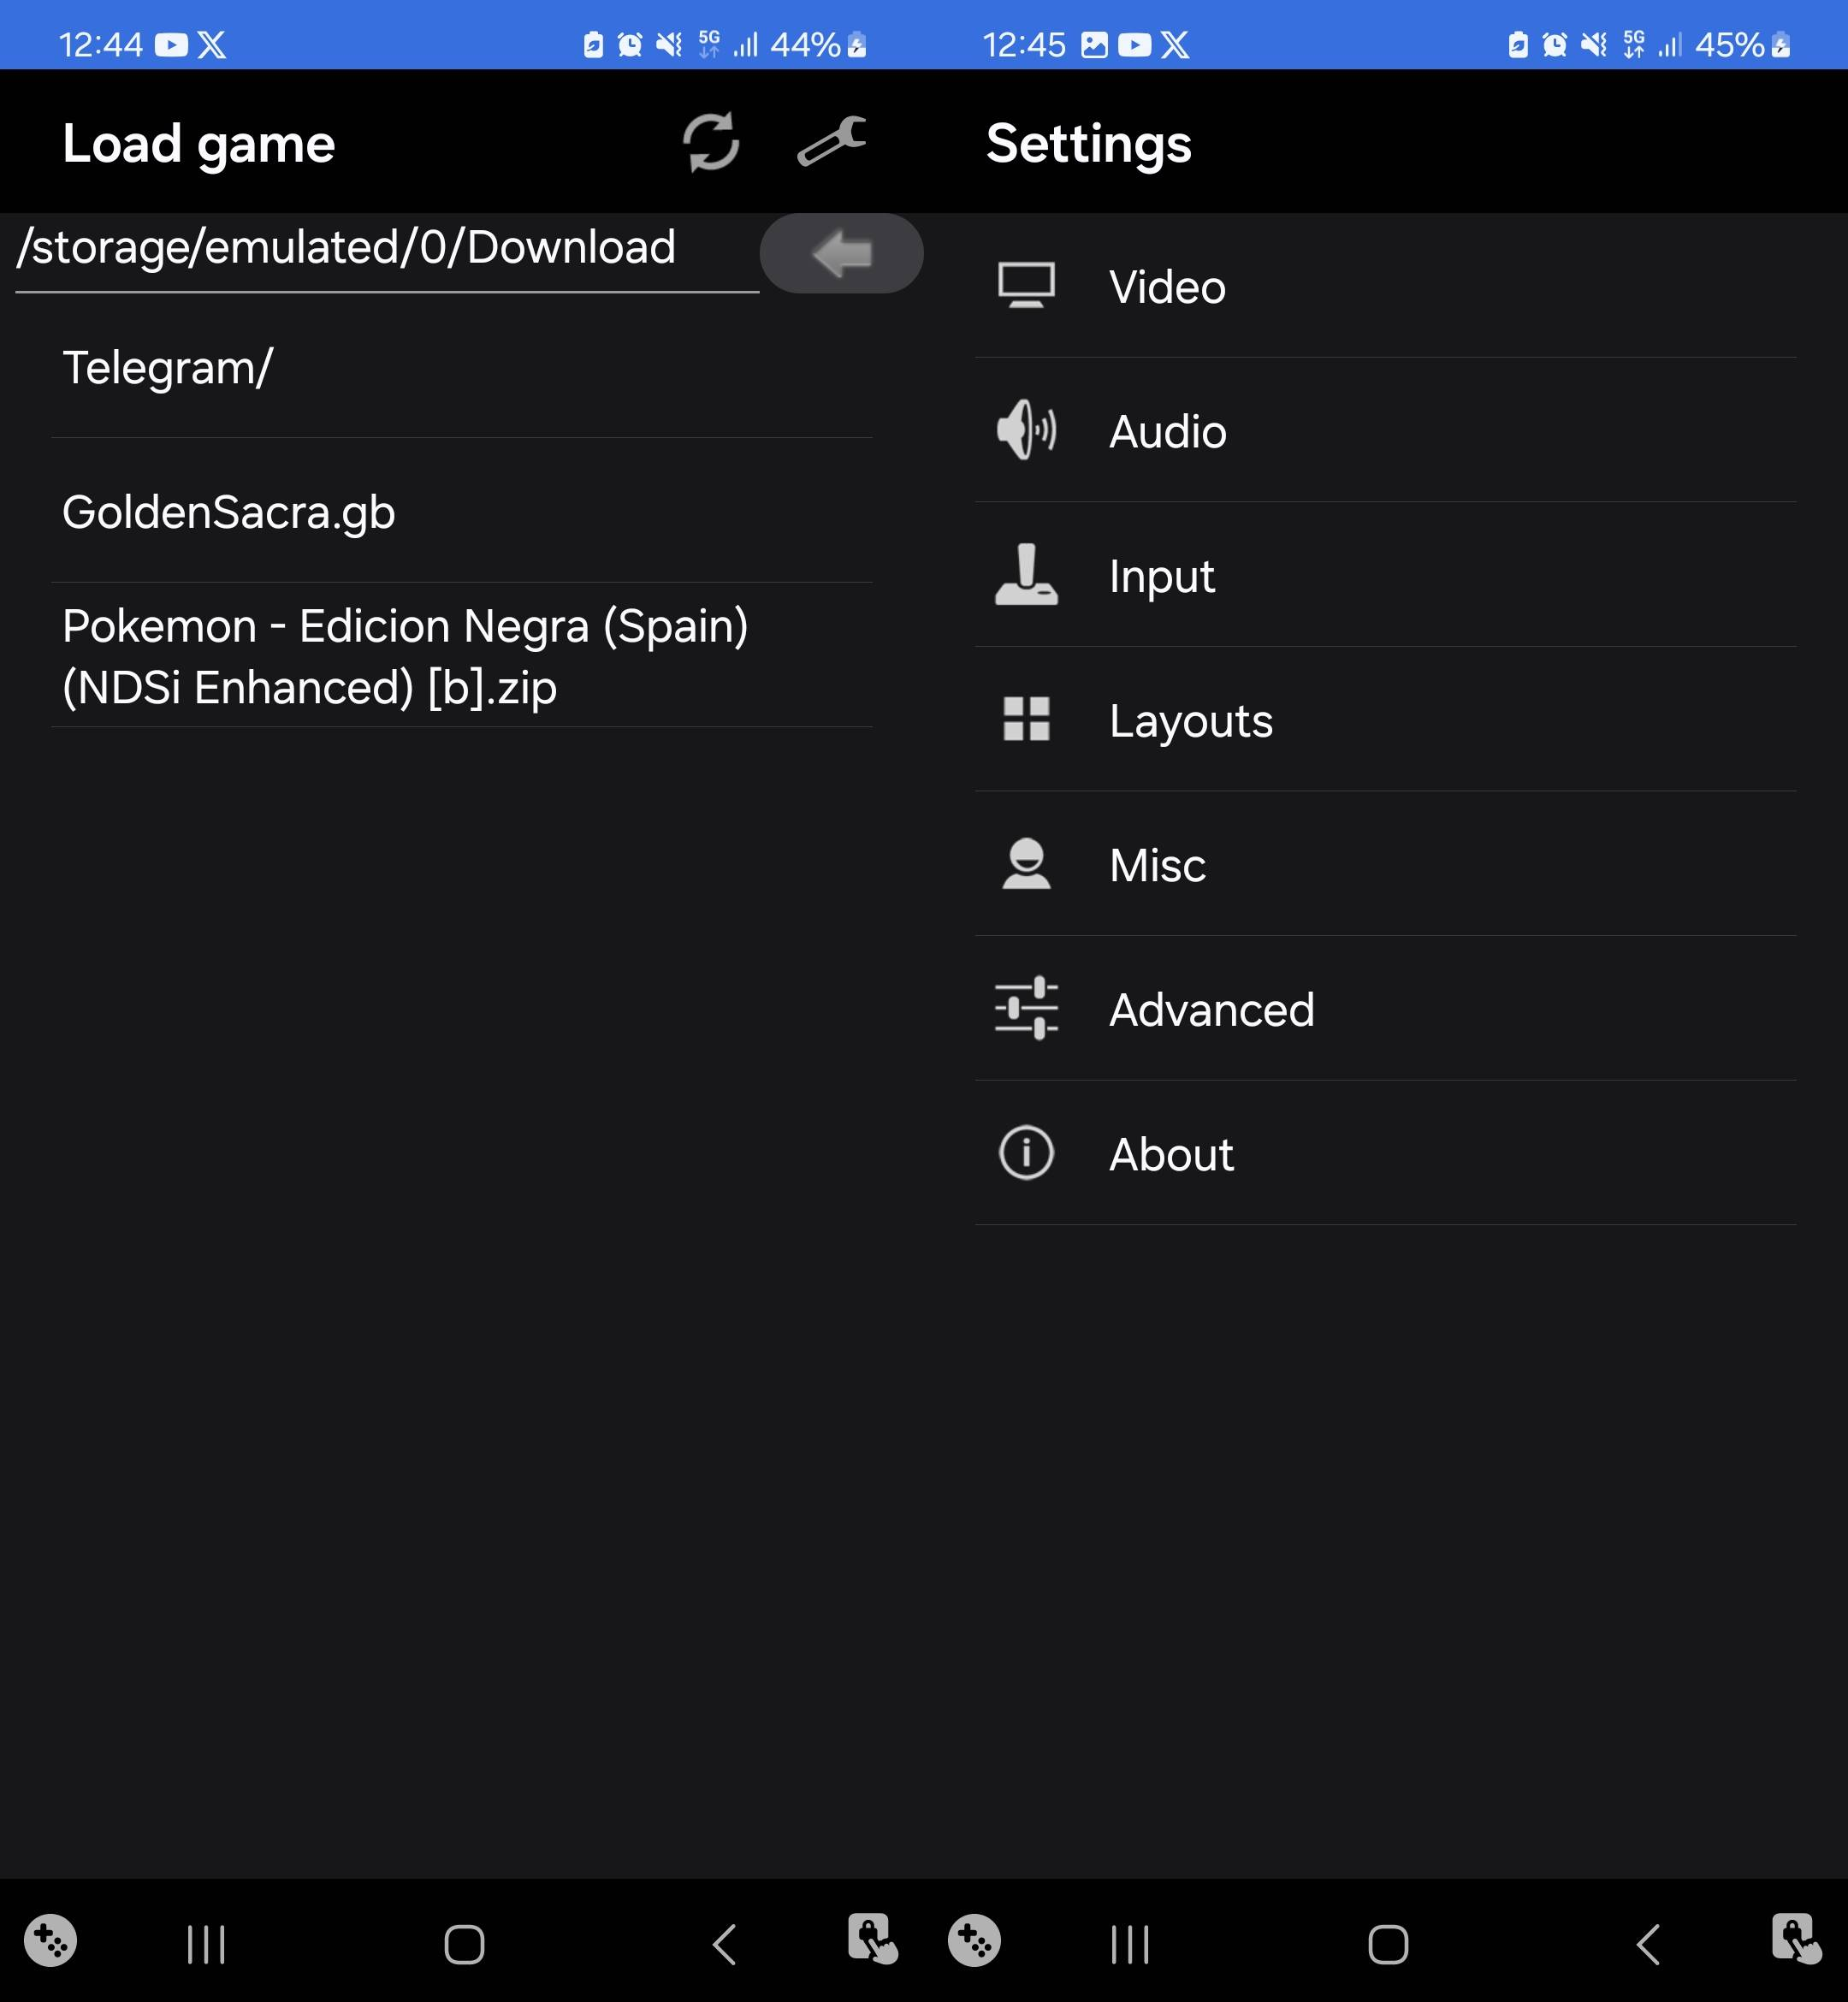
\includegraphics[width=0.55\textwidth]{include/images/myoldboy2.jpg}
    \caption{My OldBoy! - Menú de inicio y pantalla de ajustes.}
    \label{figure:oldboy2}
\end{figure}

\clearpage

La \textbf{pantalla de juego} presenta un \textbf{diseño más simplificado} en comparación con otros emuladores destacados. Su principal \textbf{ventaja} radica en la \textbf{facilidad para ajustar la posición y tamaño} de los botones, permitiendo al usuario personalizar su experiencia de juego. Sin embargo, algunos usuarios consideran que, dado que se trata de una aplicación de pago, el aspecto gráfico podría beneficiarse de mejoras adicionales para estar a la altura de sus competidores.

\begin{figure}[h]
    \centering
    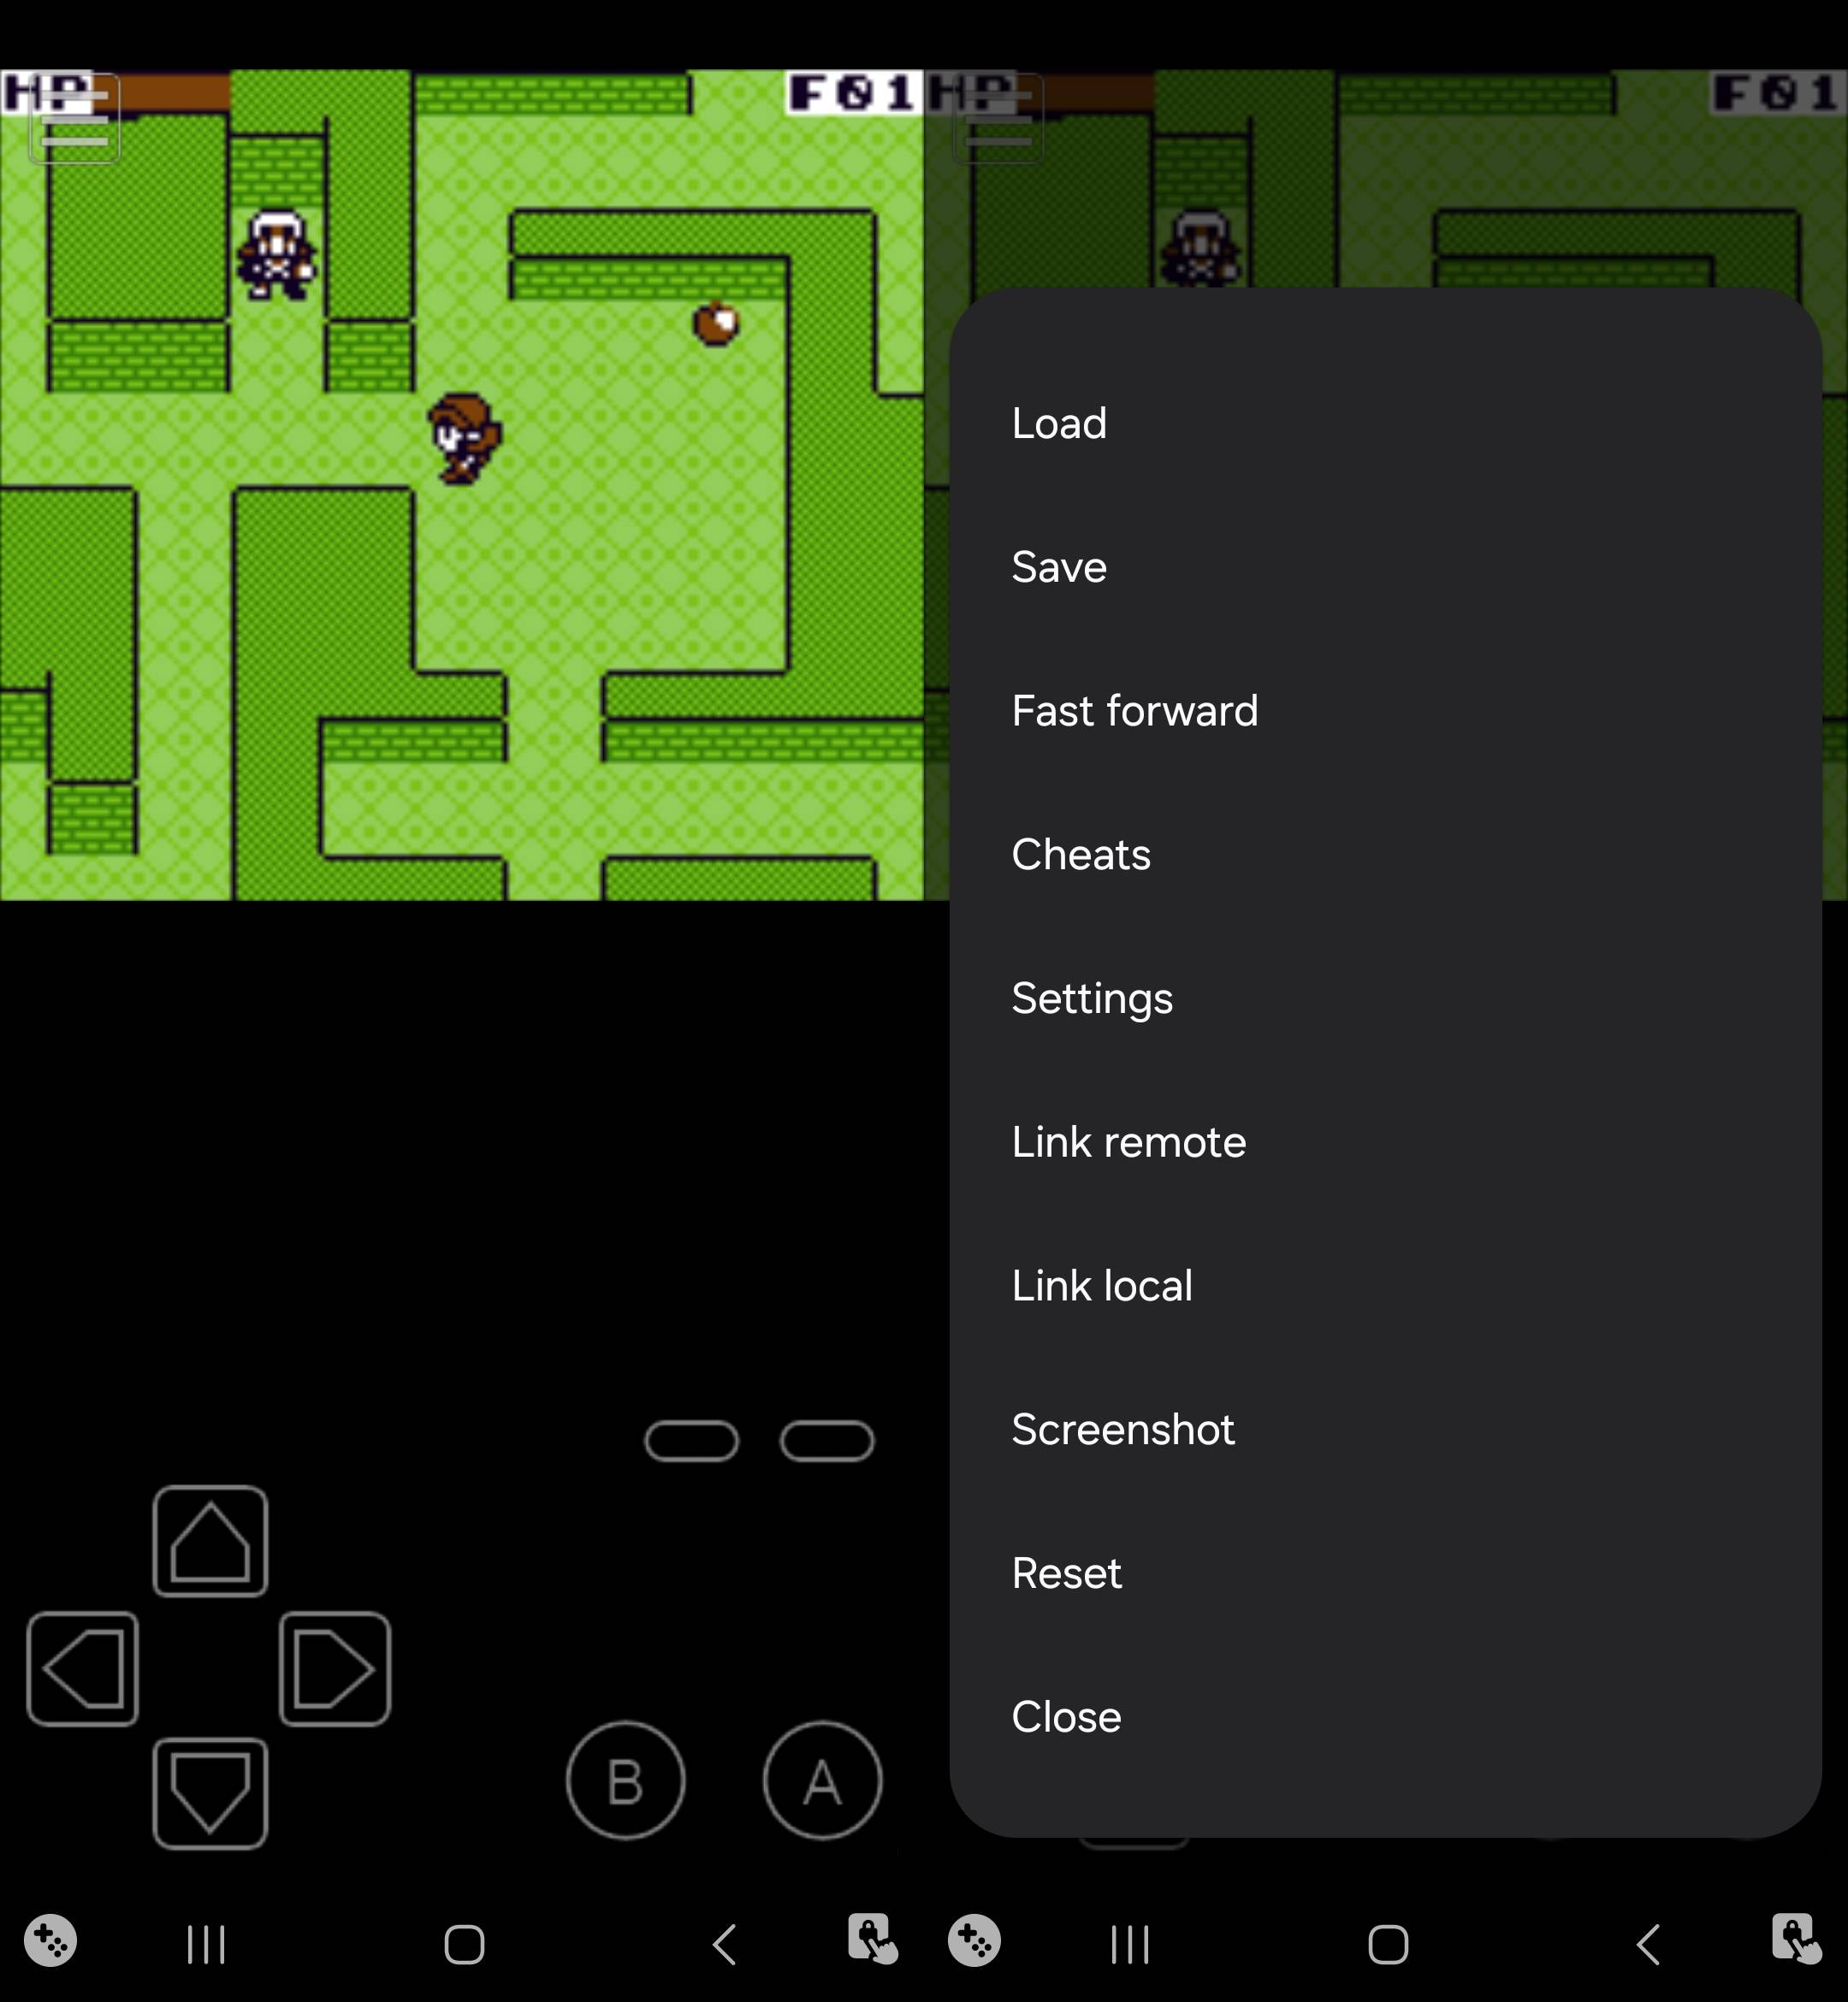
\includegraphics[width=0.65\textwidth]{include/images/myoldboy3.jpg}
    \caption{My OldBoy! - Pantalla y opciones de juego.}
    \label{figure:oldboy3}
\end{figure}
\begin{figure}[H]
    \centering
    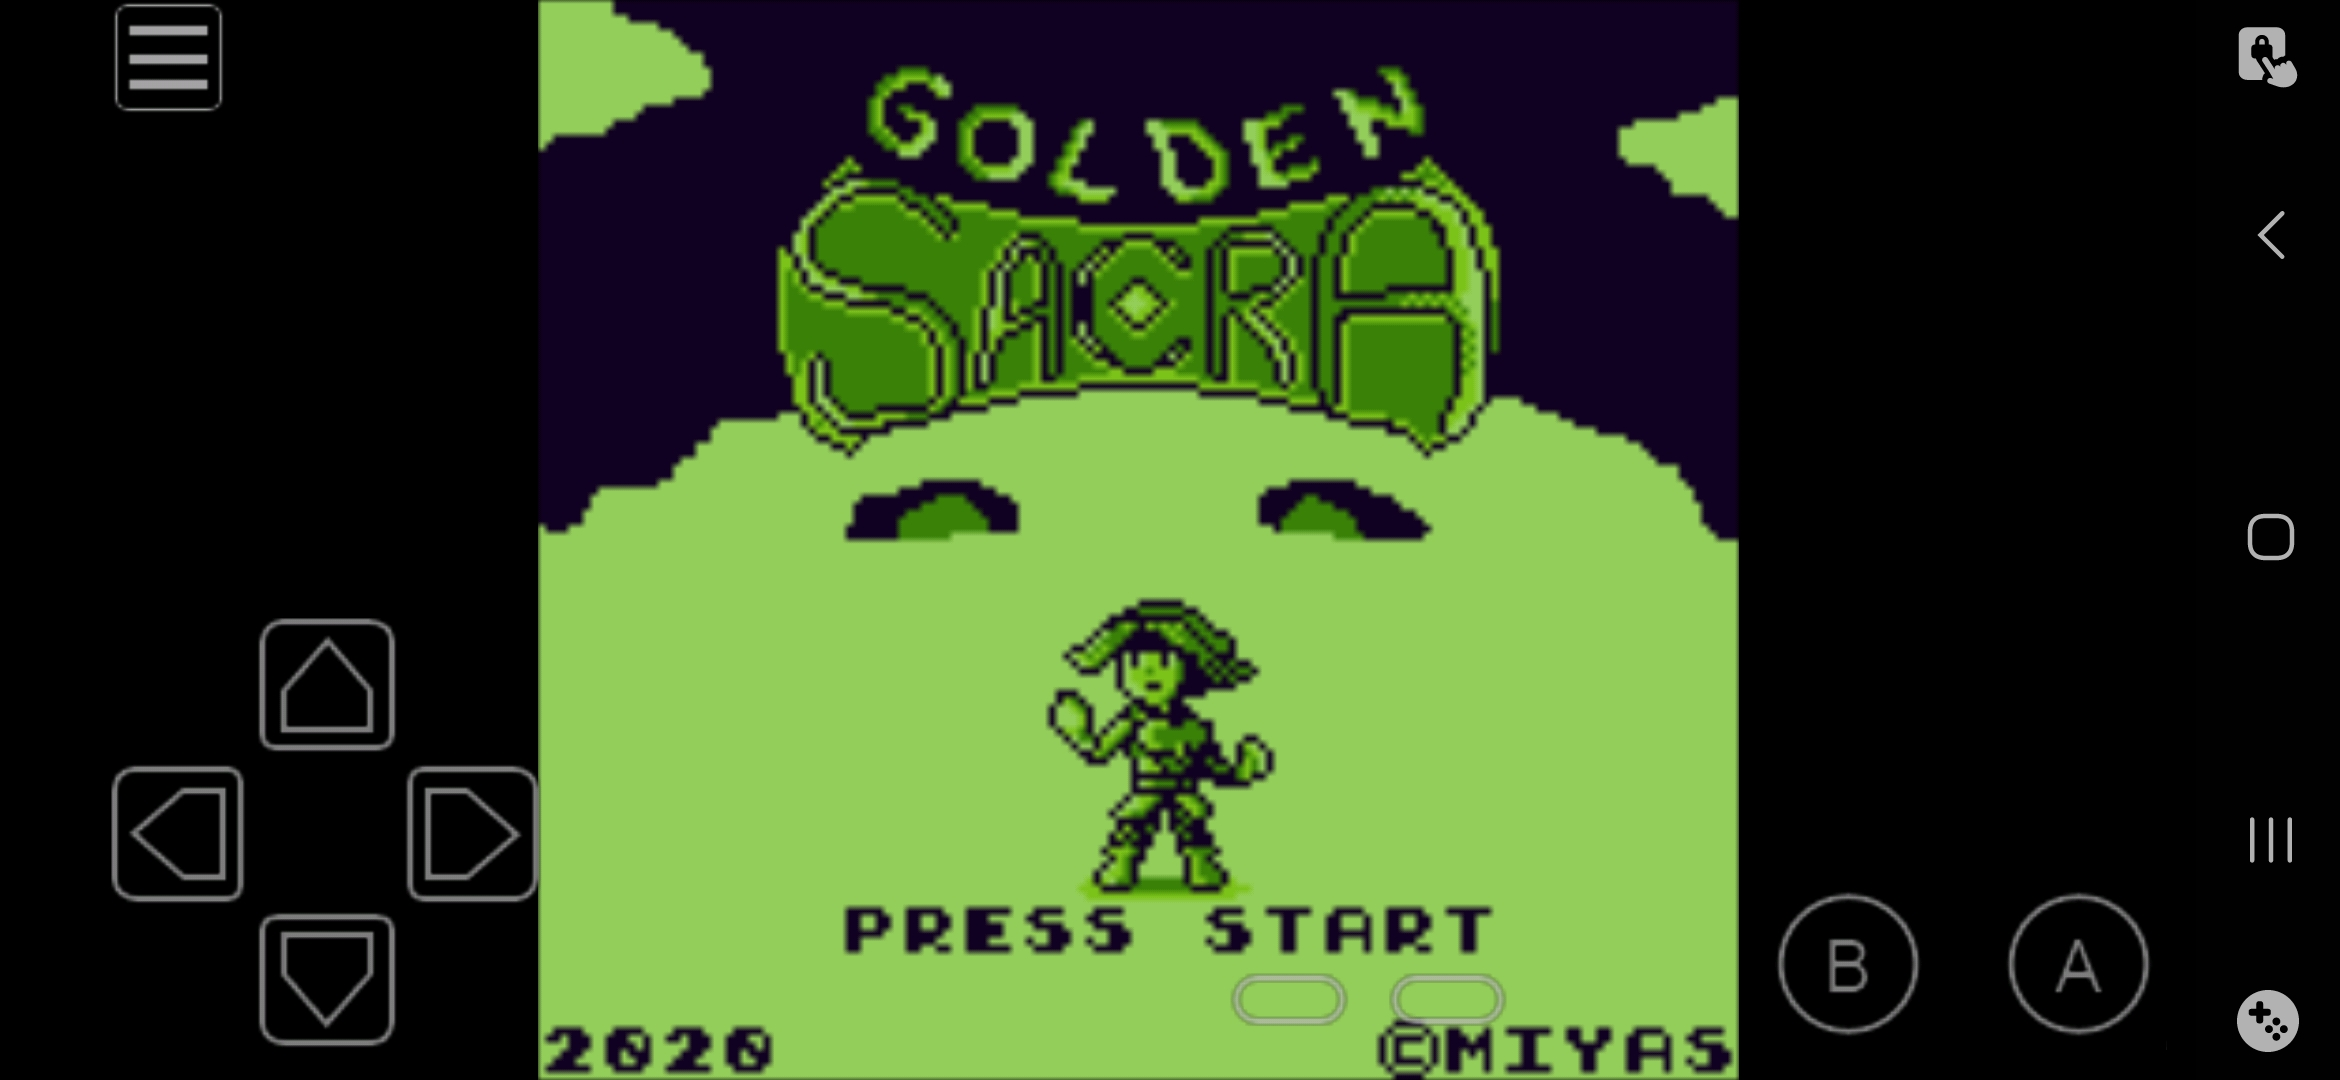
\includegraphics[width=0.65\textwidth]{include/images/myoldboyportrait.jpg}
    \caption{My OldBoy! - Pantalla de juego en orientación horizontal.}
    \label{figure:oldboy4}
\end{figure}

\clearpage

\subsubsection{GBCC}
GBCC es un \textbf{emulador multiplataforma} de Game Boy y Game Boy Color desarrollado en lenguaje C. Está disponible en Linux, Windows, Android y macOS.
\\\\
Entre sus funcionalidades se incluyen soporte para GUIs basadas en SDL y GTK, paletas personalizadas para juegos DMG, estados de guardado automáticos, y una función de turbo ajustable. También soporta shaders como Dot-Matrix y Subpixel, los cuales permiten una reproducción precisa de los colores en CGB. Además, ofrece integración con hardware como el Rumble Pak, acelerómetros y la Game Boy Printer, aunque algunos periféricos como el IR Port y el Pocket Sonar no están implementados.
\\\\
También \textbf{soporta diversos controladores de memoria: MBC1, MBC2, MBC3 y MBC5}, pero aún carece de soporte para MBC6 y MBC7, entre otros. Además, el emulador tiene la \textbf{capacidad de simular el cable link}, aunque es una conexión \textit{fake} consigo mismo.
\\\\
El proyecto se destaca por su compatibilidad con shaders y la posibilidad de visualizar los datos de VRAM en una ventana separada, lo cual es útil para desarrolladores y aficionados que quieran inspeccionar los gráficos en detalle.

\begin{figure}[h]
    \centering
    
\includegraphics[width=0.6\textwidth]{include/images/gbcclogo.png}
    \caption{GBCC - Logotipo.}
    \label{figure:gbcclogo}
\end{figure}

La \textbf{pantalla de juego} se caracteriza por su \textbf{diseño minimalista y adaptable}. Dependiendo de si se carga una ROM de Game Boy (DMG) o de Game Boy Color (CGB), la interfaz ajusta su apariencia para emular de manera más fiel las características visuales de la consola correspondiente. El diseño de los controles también \textbf{se adapta dinámicamente a las dimensiones del dispositivo}: en modo vertical, la separación entre los botones y la escala de la pantalla gráfica varían según el ancho y el alto disponibles. En el modo horizontal, el diseño se ajusta automáticamente, manteniendo la proporción y los colores, sin perder la coherencia visual. Además, se pueden observar \textbf{características adicionales} como el \textbf{botón de turbo} y la \textbf{aplicación de shaders} como el Dot-Matrix para mejorar la experiencia visual.
\\\\
Por último, GBCC \textbf{permite personalizar el fondo de pantalla} que simula la consola original, brindando la opción de cambiar el color según las preferencias del usuario, lo que añade un toque personal a la experiencia de emulación. Esta característica es muy apreciada por quienes buscan una mayor personalización en la interfaz.

\begin{figure}[h]
    \centering
    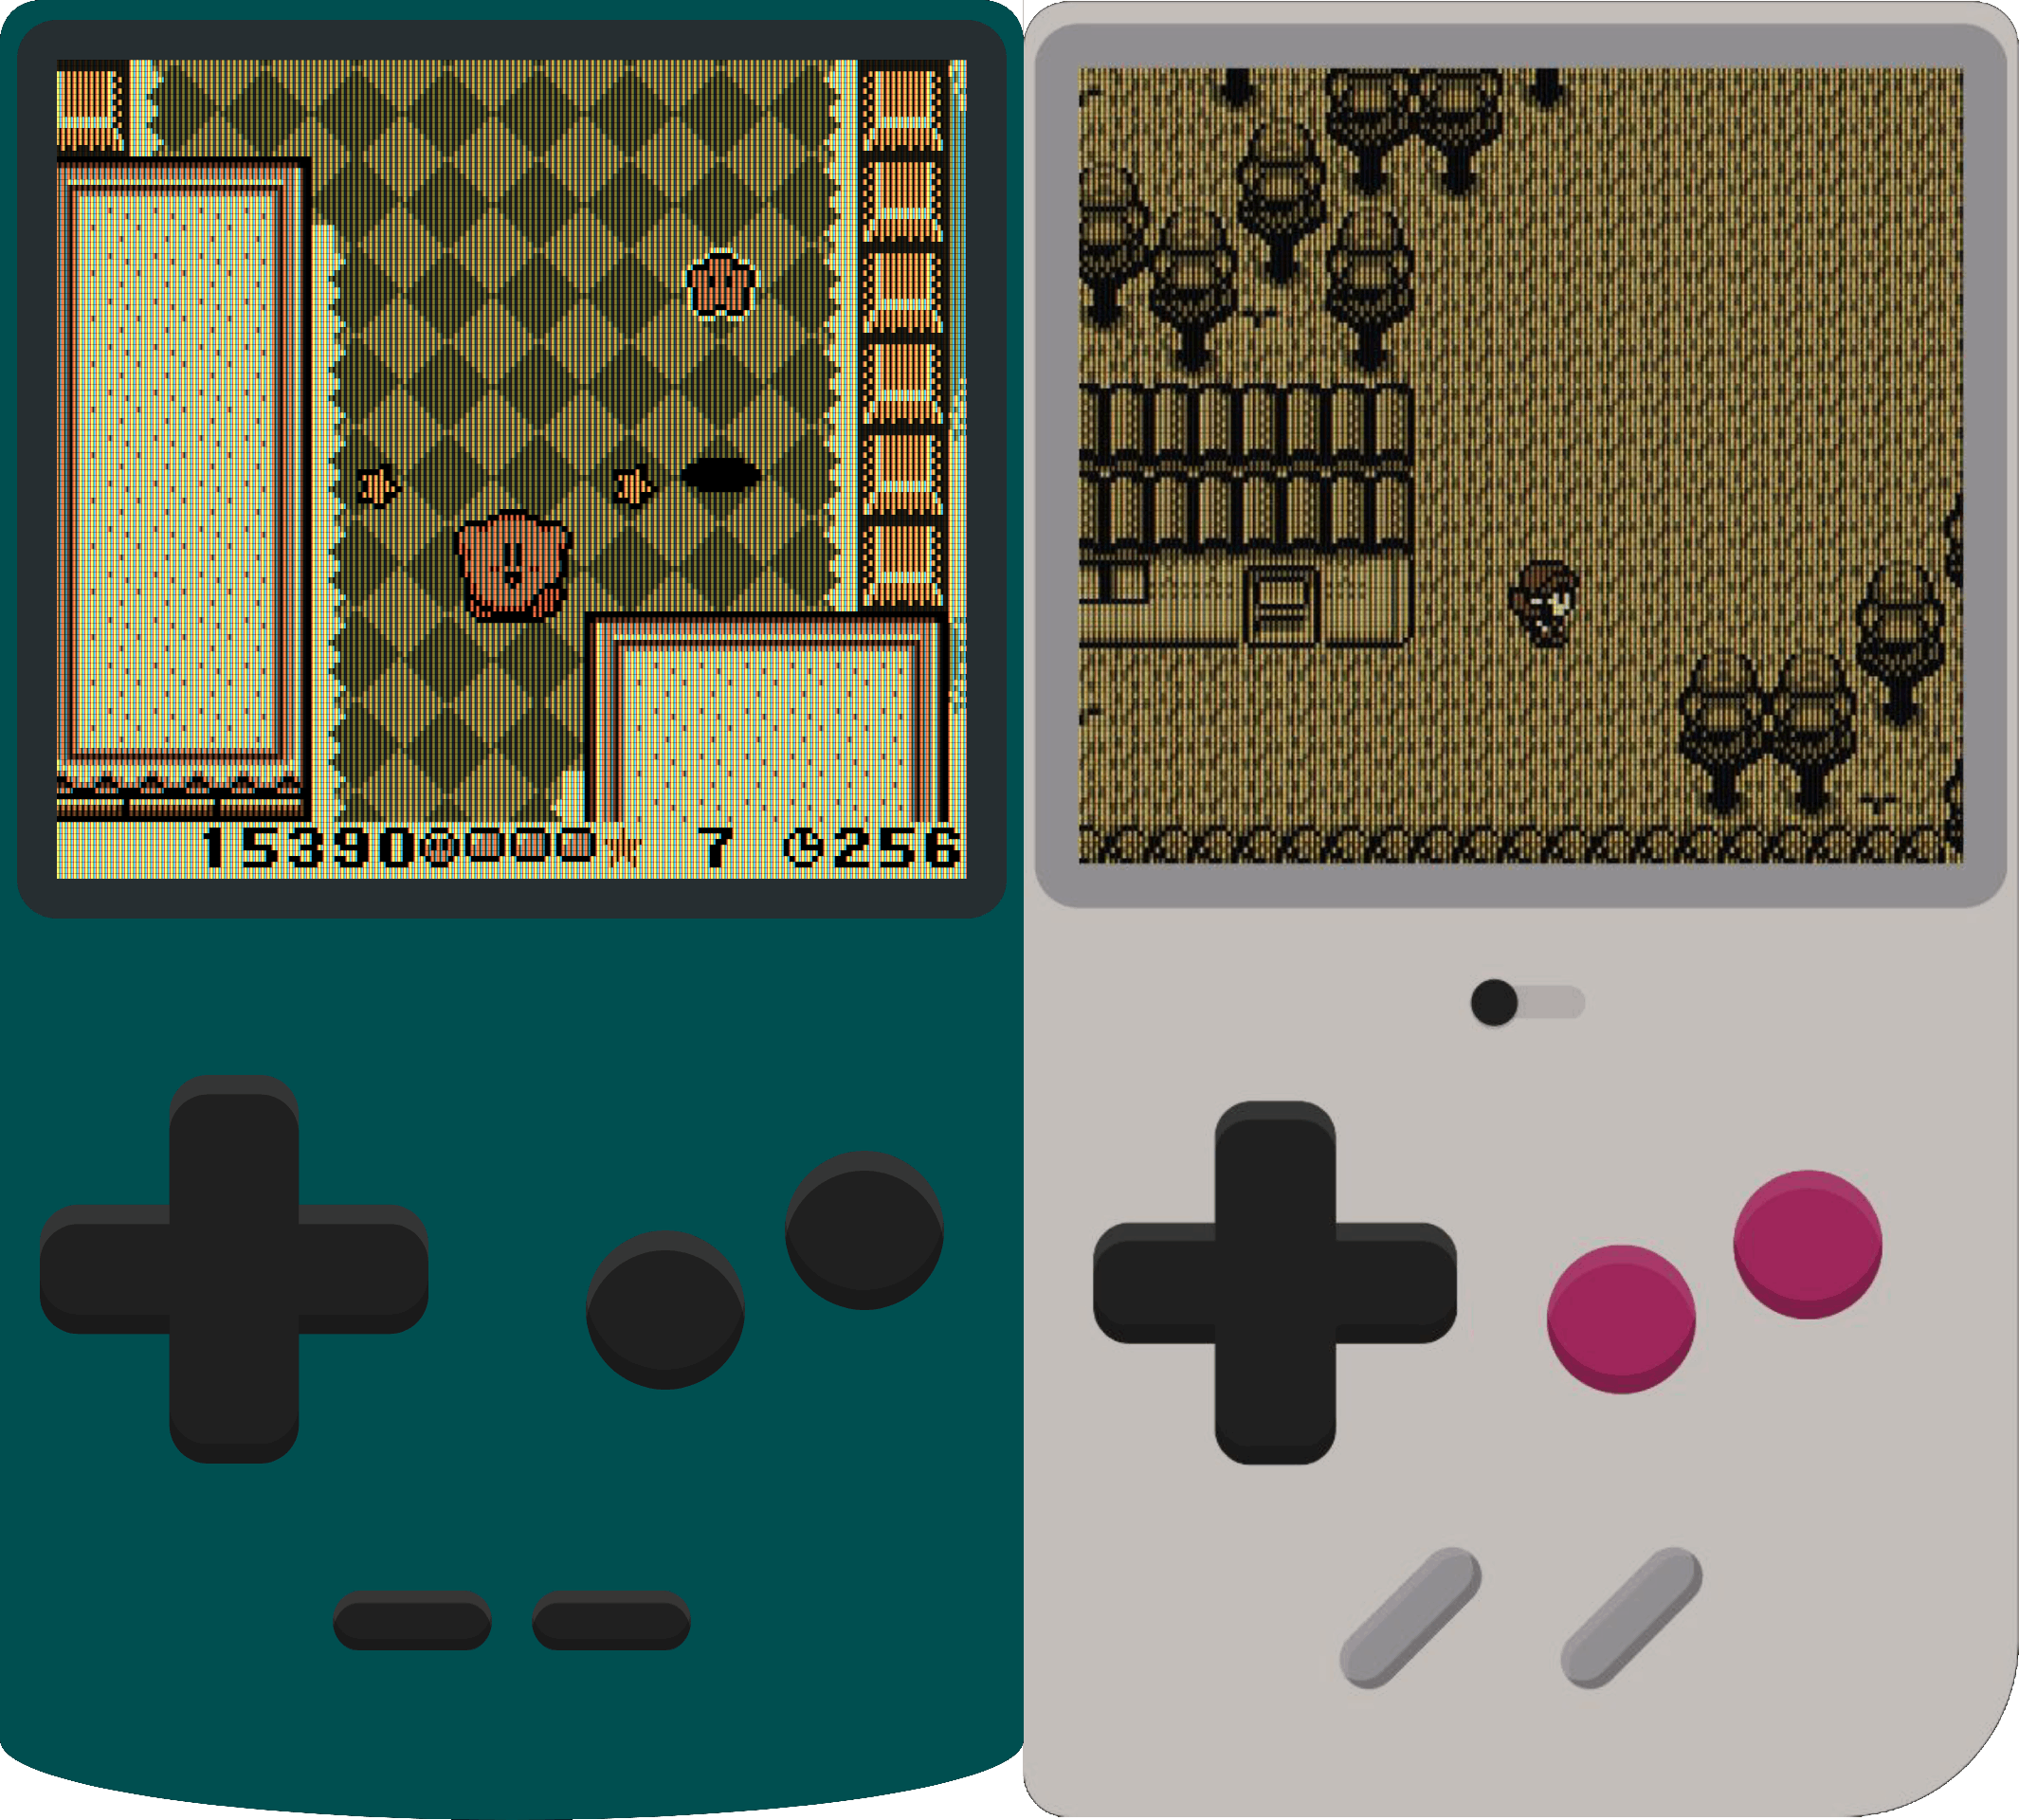
\includegraphics[width=0.6\textwidth]{include/images/gbccgame.png}
    \caption{GBCC - Pantalla de juego.}
    \label{figure:gbccgame}
\end{figure}

\begin{figure}[h]
    \centering
    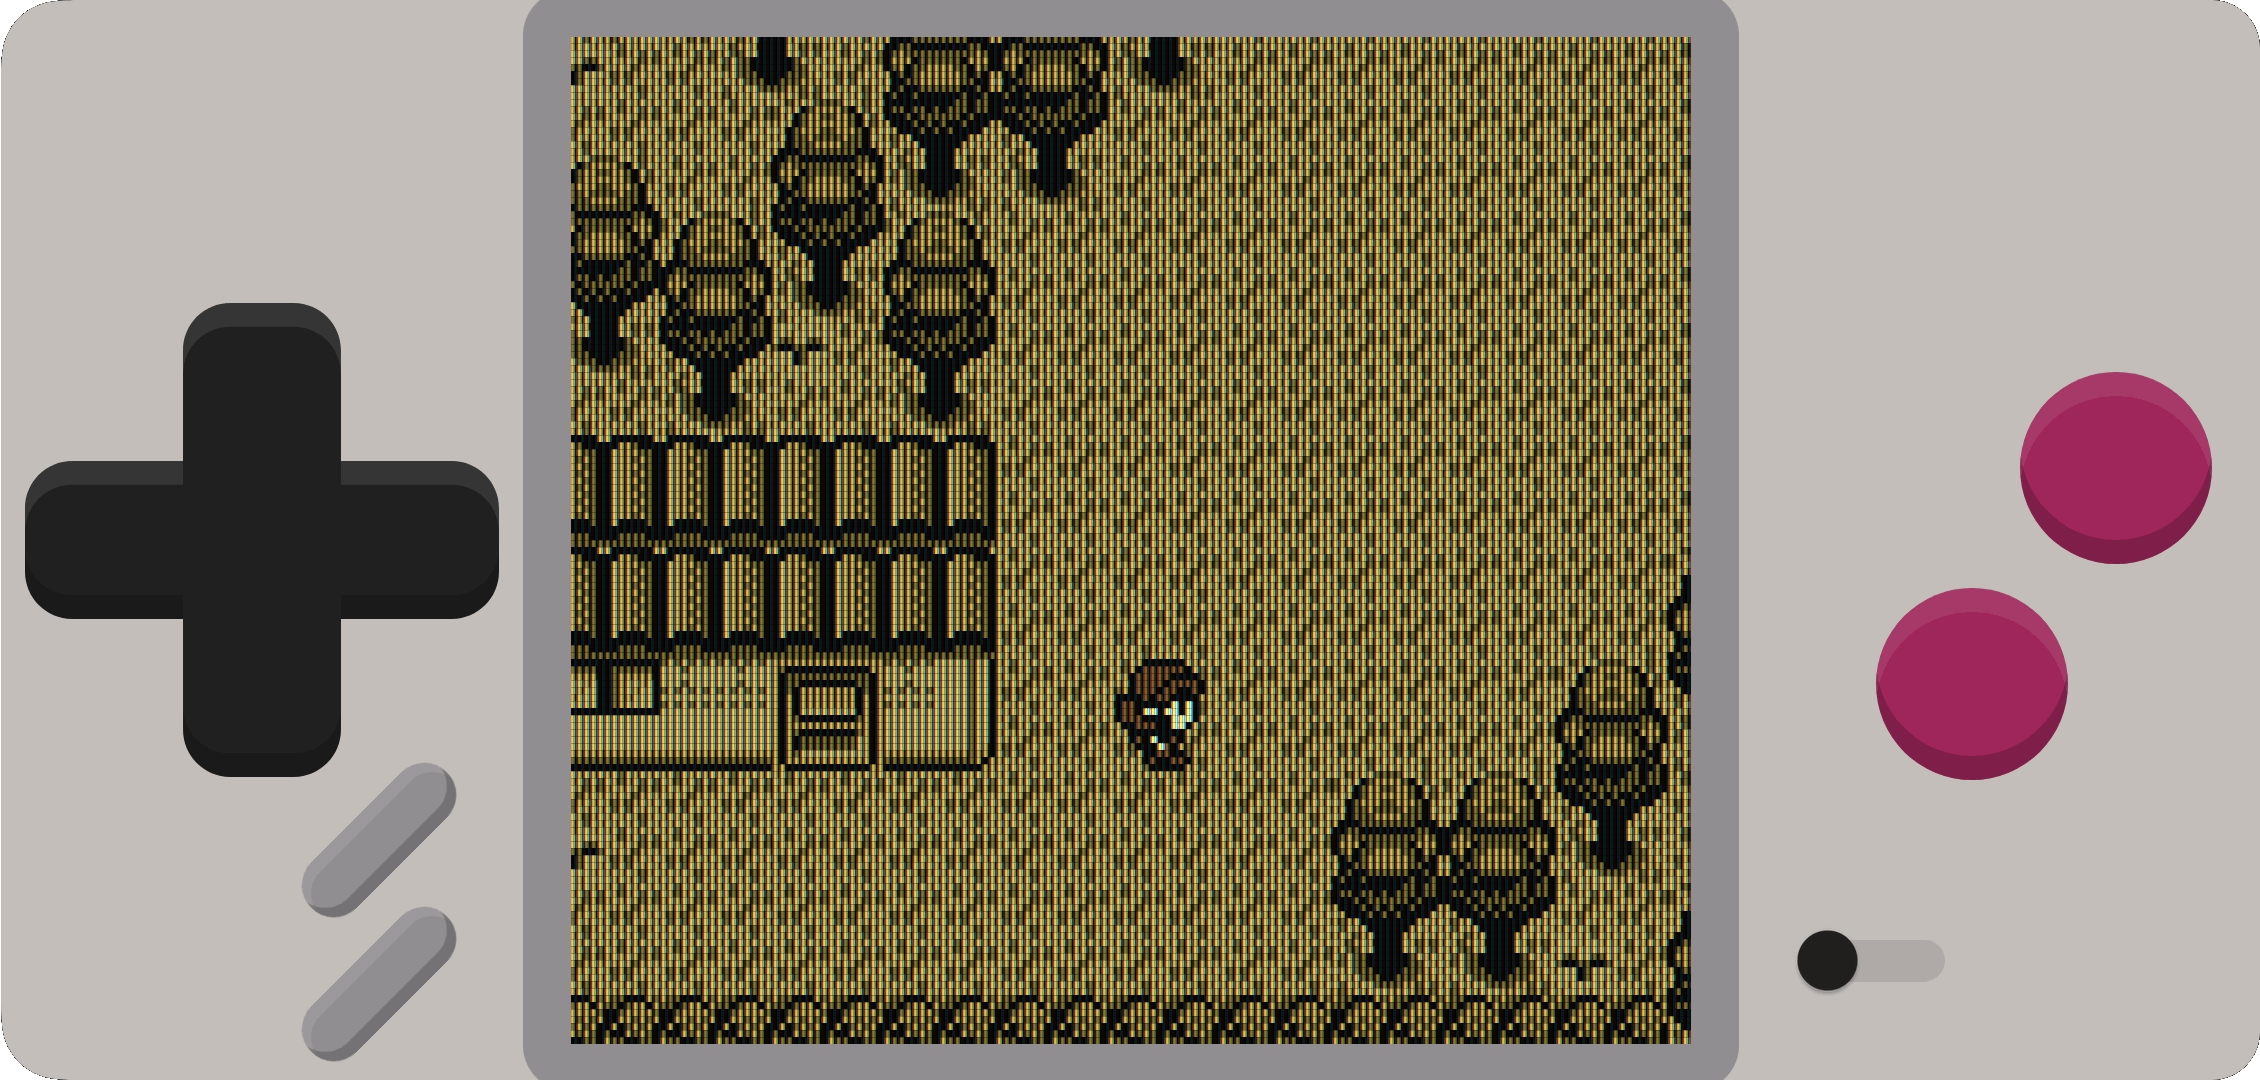
\includegraphics[width=0.6\textwidth]{include/images/gbccgameportrait.png}
    \caption{GBCC - Pantalla de juego en orientación horizontal.}
    \label{figure:gbccgameportrait}
\end{figure}

\clearpage

\subsubsection{iGBA}

El emulador iGBA fue una aplicación \textbf{diseñada para dispositivos iOS}, disponible brevemente en la App Store antes de ser \textbf{retirada en abril de 2024}. Permitía a los usuarios emular juegos de Game Boy, Game Boy Color y Game Boy Advance en sus iPhones, ofreciendo características como guardado de estado, avance rápido y soporte para ROMs legalmente adquiridas.
\\\\
Entre sus características principales destacaban la \textbf{capacidad de guardar estados de juego}, permitiendo a los usuarios guardar y retomar partidas en cualquier momento, además de la \textbf{función de avance rápido} (igual que GBCC), que permitía saltar rápidamente escenas o partes lentas del juego. Sin embargo, un detalle a mejorar era que esta velocidad del avance era excesivamente rápida y no permitía ajustes más finos.

\begin{figure}[h]
    \centering
    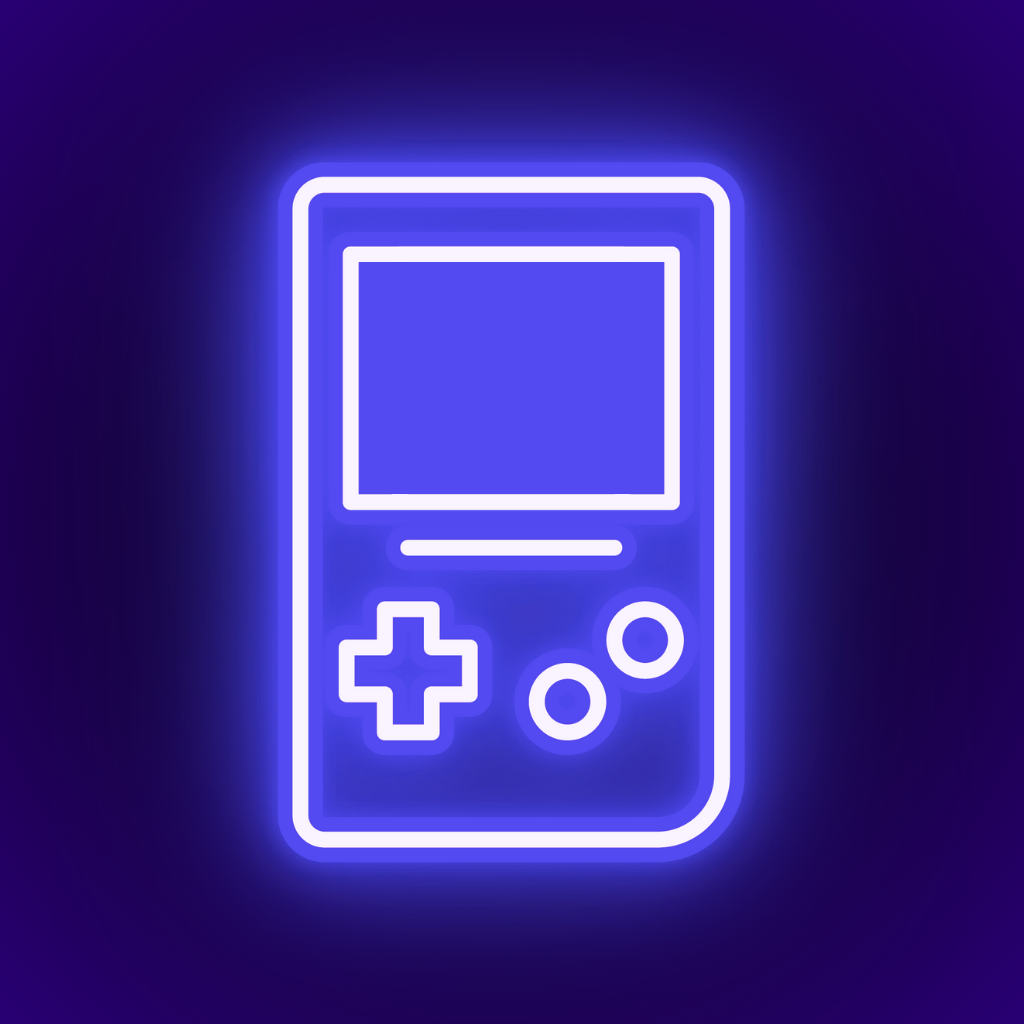
\includegraphics[width=0.3\textwidth]{include/images/igbalogo.png}
    \caption{iGBA - Logotipo.}
    \label{figure:igbalogo}
\end{figure}

La \textbf{interfaz} era \textbf{sencilla}, con un diseño limpio que simulaba los botones de las consolas originales. Sin embargo, \textbf{generó controversia} por dos razones: i\textbf{ncluir anuncios que interrumpían la experiencia de juego y ser una copia no autorizada de GBA4iOS}, un emulador desarrollado por \textit{Riley Testut}. Este conflicto con el código de GBA4iOS, junto con la preocupación por la privacidad y la recopilación de datos de los usuarios, llevó a críticas dentro de la comunidad de emuladores​.
\\\\
Los controles virtuales incluían botones de hombro para los juegos de Game Boy Advance, aunque algunos usuarios mencionaron que estos botones eran algo pequeños. Además, ofrecía un menú de opciones en la esquina inferior izquierda con funciones como guardado rápido, carga de estados, códigos de trucos y avance rápido.
\\\\
A pesar de sus problemas, algunos usuarios apreciaron lo fácil que era configurarlo y su capacidad para emular juegos retro sin retrasos significativos.

\begin{figure}[h]
    \centering
    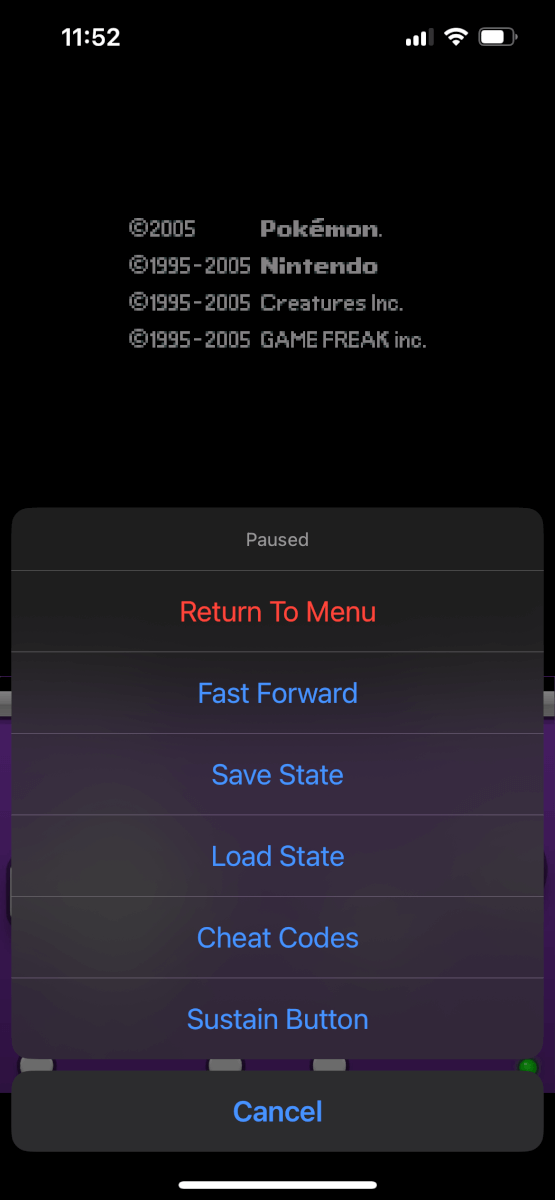
\includegraphics[width=0.25\textwidth]{include/images/igbasettings.PNG}
    \caption{iGBA - Ajustes de juego.}
    \label{figure:igbasettings}
\end{figure}

\begin{figure}[h]
    \centering
    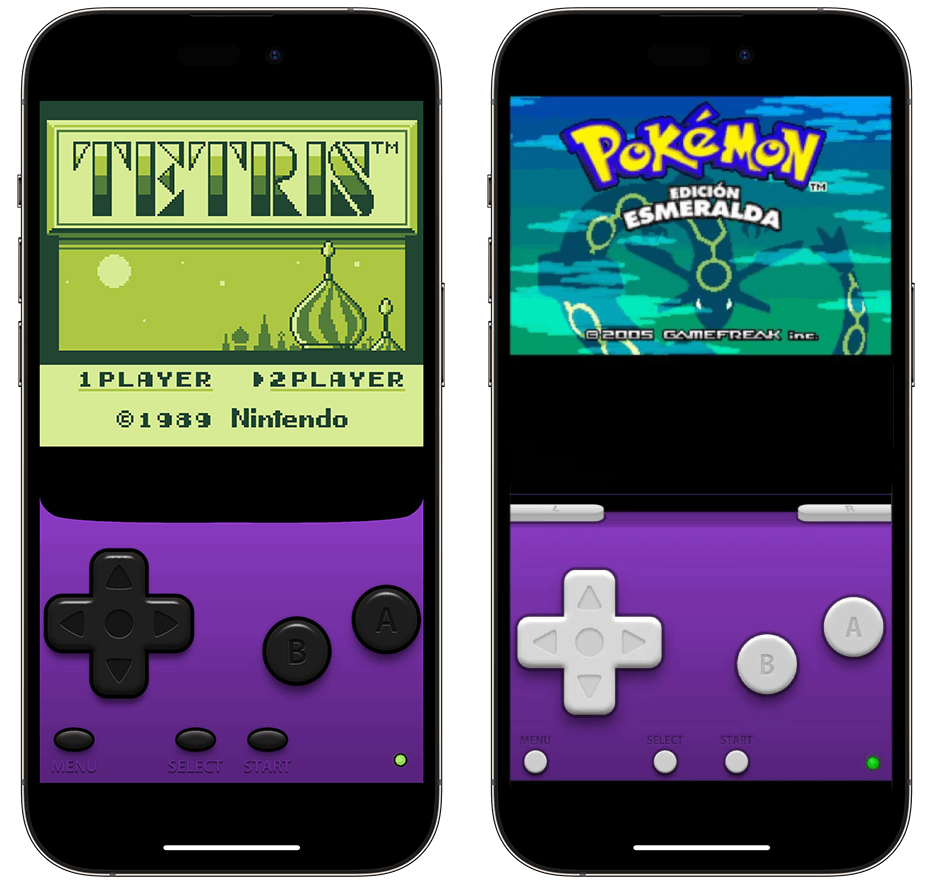
\includegraphics[width=0.65\textwidth]{include/images/iGBAgame.png}
    \caption{iGBA - Pantalla de juego.}
    \label{figure:igbagame}
\end{figure}


\cleardoublepage

\chapter{Análisis y Diseño}
\label{design}

Este capítulo recoge el proceso de \textbf{análisis y diseño} previo al desarrollo del emulador, donde se definen los \textbf{requisitos que debe cumplir la aplicación} y se plantean las primeras decisiones estructurales y visuales del proyecto.
\\\\
En primer lugar, se detallan los \textbf{requisitos funcionales y no funcionales}, los cuales especifican tanto las funcionalidades que debe ofrecer la aplicación como las restricciones de calidad, rendimiento o usabilidad que debe respetar. A continuación, se presentan los \textbf{casos de uso}, acompañados de su correspondiente diagrama, para ilustrar de manera clara la interacción entre el usuario y el sistema.
\\\\
Finalmente, se incluyen una \textbf{serie de mockups} que representan visualmente la interfaz de usuario en sus distintas pantallas, ayudando a anticipar la experiencia del usuario final y facilitando una primera validación del diseño.

\section{Requerimientos}

A continuación se detallan los \textbf{requerimientos funcionales y no funcionales} que rigen el diseño y la implementación del proyecto. Estos requerimientos han sido definidos a partir del análisis de las necesidades del usuario final y de las restricciones técnicas:

\subsection{Requerimientos Funcionales}

Estos requerimientos son las \textbf{capacidades específicas que la aplicación debe cumplir} para garantizar que su funcionamiento sea acorde a los objetivos establecidos:

\begin{itemize}
    \item \textbf{Carga de ROMs}: El usuario debe poder seleccionar y cargar archivos .gb o .gbc desde su dispositivo.
    \item \textbf{Emulación}: Debe replicar fielmente el comportamiento del hardware original.
    \item \textbf{Interfaz táctil}: Proveer botones virtuales que simulen los originales.
    \item \textbf{Audio}: Emular el sonido original de la consola.
    \item \textbf{Gestión de estado}: Guardar y cargar partidas.
    \item \textbf{Compatibilidad}: Dar soporte para ROMs de DMG y CGB.
    \item \textbf{Configuraciones}: Permitir al usuario ajustar las características del emulador, como la velocidad y los controles.
\end{itemize}

\subsection{Requerimientos No Funcionales}

Estos requerimientos se enfocan en \textbf{aspectos de calidad de la aplicación}, como el rendimiento o la usabilidad, con el objetivo de asegurar una experiencia fluida y eficiente.

\begin{itemize}
    \item \textbf{Rendimiento}: La emulación debe ir a la frecuencia original de la consola en la mayoría de los dispositivos Android.
    \item \textbf{Compatibilidad}: Funcionar en dispositivos Android 8.0 o superior.
    \item \textbf{Eficiencia}: Consumo de batería optimizado durante la ejecución.
    \item \textbf{Usabilidad}: La interfaz debe ser intuitiva y accesible para el usuario.
    \item \textbf{Mantenimiento}: Código modular, que sea fácil de escalar y el cual disponga de una buena documentación para facilitar futuras mejoras.
\end{itemize}

\section{Casos de Uso}

Los casos de uso permiten \textbf{identificar y documentar cómo los usuarios interactuarán con el sistema}, destacando las funcionalidades clave y sus flujos de ejecución.

\begin{figure}[H]
    \centering
    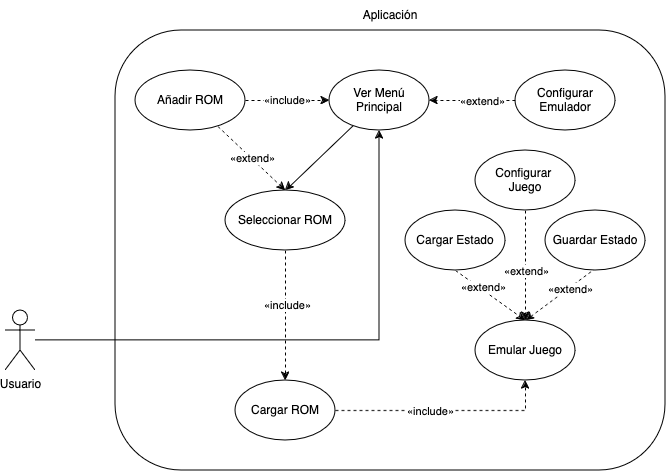
\includegraphics[width=0.7\textwidth]{include/images/casosuso.png}
    \caption{Diagrama de Casos de Uso}
    \label{figure:usecases}
\end{figure}

El usuario tiene \textbf{acceso directo al menú principal} al entrar en la aplicación. Desde ahí, el usuario puede realizar diferentes acciones como \textbf{añadir o seleccionar una ROM o configurar de forma general el emulador}. La selección de una ROM incluye los procesos de carga y emulación. Además, durante la emulación, el usuario \textbf{puede cargar o guardar el estado y configurar el juego}. Las relaciones entre los casos de uso se estructuran con inclusiones para acciones necesarias y extensiones para funcionalidades opcionales.

\section{Mockup}

La aplicación seguirá un \textbf{diseño minimalista}, tomando como \textbf{referencia principal} el emulador \textbf{GBCC}. En su versión inicial, el \textbf{menú principal} presentará una \textbf{lista en formato de cuadrícula} que mostrará todas las ROMs agregadas por el usuario. Cada uno de los elementos de la cuadrícula contará con una \textbf{imagen predeterminada}, representando la consola original, ya sea DMG o CGB, junto con el nombre de la ROM. Estas \textbf{se ordenarán alfabéticamente} para facilitar la navegación. Este enfoque busca mantener una interfaz limpia y funcional, con un acceso directo a los juegos.
\\\\
En la \textbf{barra de navegación} se mostrarán \textbf{dos íconos}. El primero, representado por un símbolo de \textbf{suma} ("+"), permitirá al usuario \textbf{agregar nuevas ROMs} a la aplicación. El segundo ícono, con la forma de un \textbf{engranaje}, brindará acceso a la \textbf{configuración general} del emulador, que incluirá opciones relacionadas con el video, audio, disposición de controles, entre otros. Estas configuraciones tendrán un impacto en todos los juegos de manera uniforme.
\\\\
\textbf{La imagen} de cada juego \textbf{podrá ser personalizada} por el usuario a través de un gesto táctil de "hold". Al realizar este gesto sobre una cuadrícula específica, el usuario tendrá la capacidad de acceder a los ajustes individuales del juego, donde podrá reemplazar la imagen predeterminada por una de su elección o modificar el nombre del juego.

\begin{figure}[h]
    \centering
    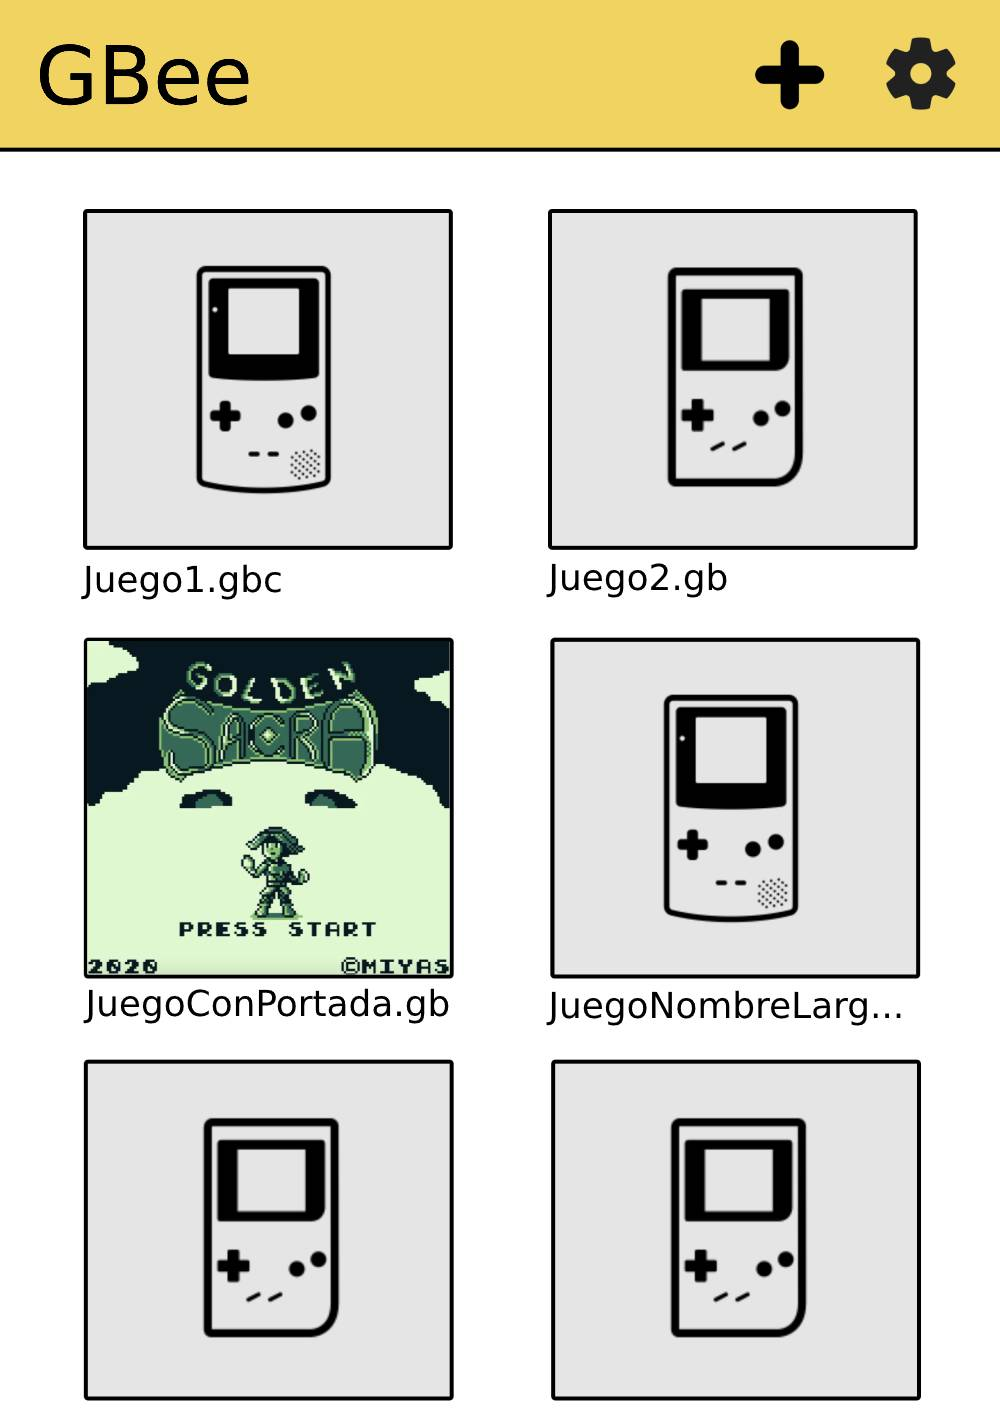
\includegraphics[width=0.4\textwidth]{include/images/mockup_menu.jpg}
    \caption{Menú de inicio.}
    \label{figure:mockupmenu}
\end{figure}

En cuanto a la pantalla de juego, se busca crear un \textbf{diseño que evoque la estética de la consola original}. Se incluirá un botón que brindará acceso a los ajustes del juego, el cual se ubicará, de manera provisional, en la parte superior izquierda de la pantalla. El layout será \textbf{minimalista}, permitiendo a los usuarios ajustar el tamaño, color y disposición de los botones según sus preferencias. La imagen de fondo tendrá un color amarillo por defecto, pero los usuarios también \textbf{podrán personalizarla a su gusto}. Además, se ofrecerá la opción de subir imágenes propias para reemplazar los botones o el fondo, lo que facilitará una experiencia de juego más personalizada y adaptada a los gustos individuales.
\\\\
Aunque no se representa en los mockups, se planea implementar un shader Dot-Matrix, similar al utilizado en GBCC. Esta función podrá desactivarse desde los ajustes generales de la aplicación.

\begin{figure}[h]
    \centering
    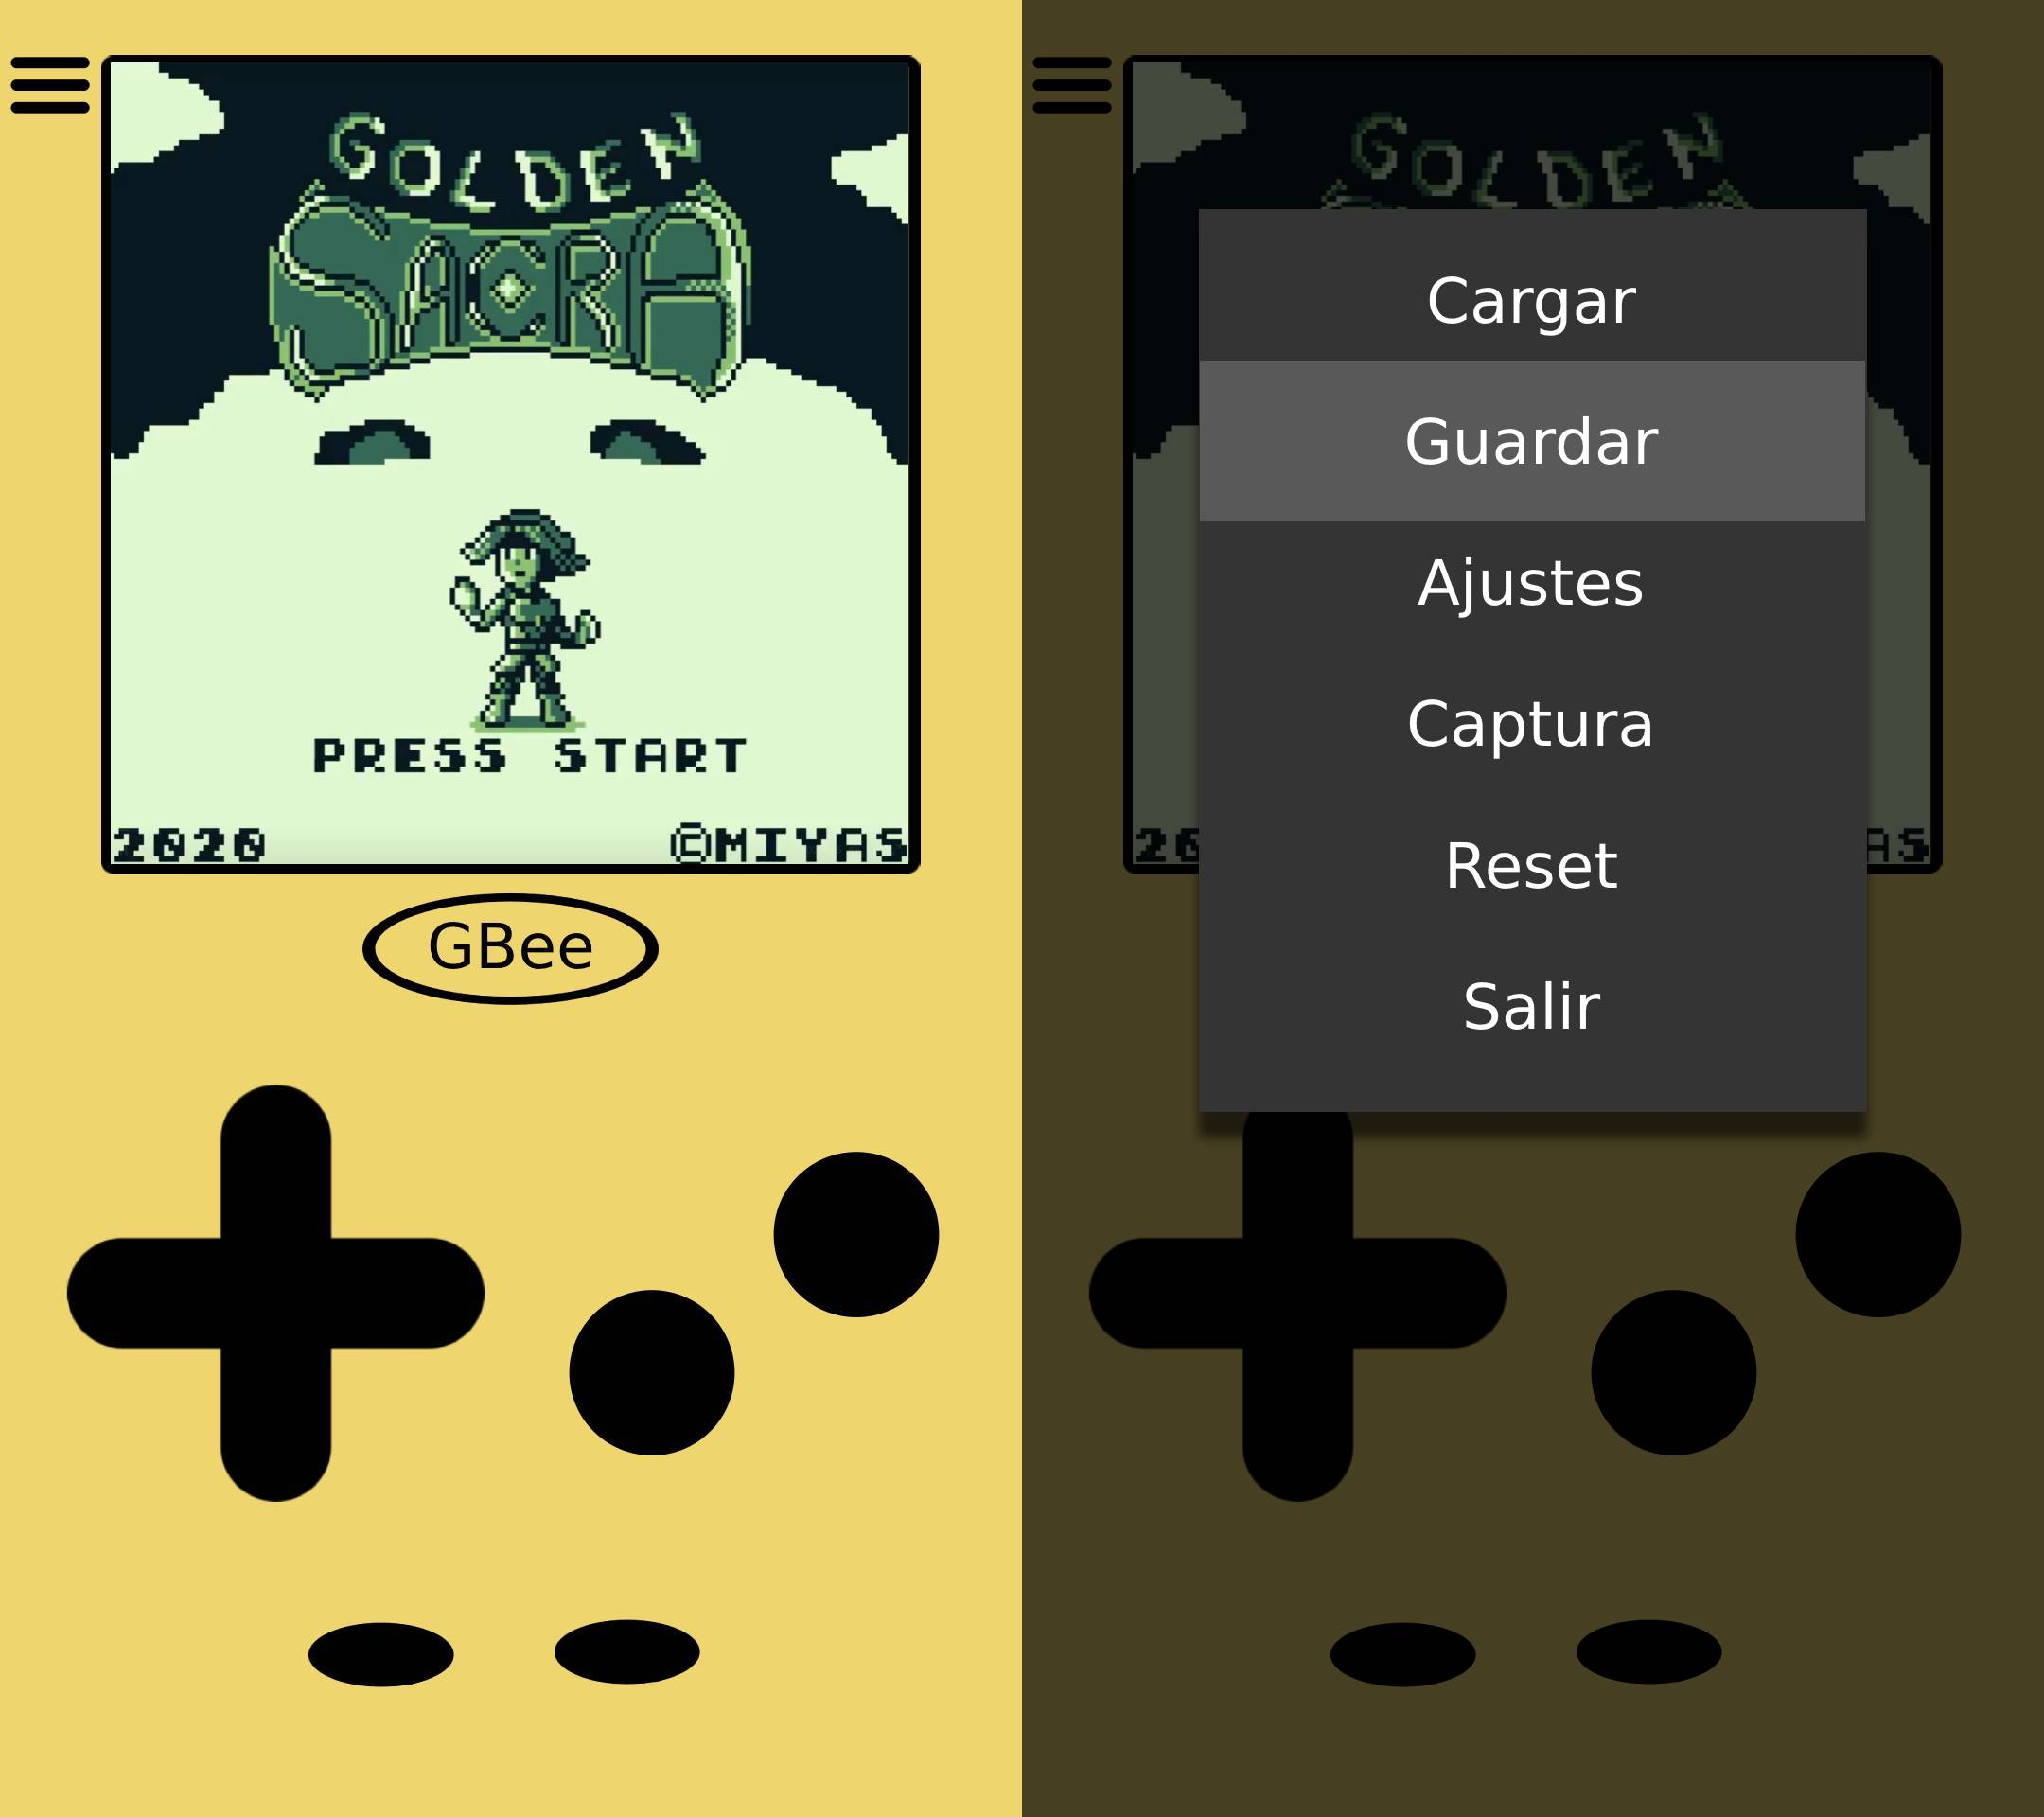
\includegraphics[width=0.6\textwidth]{include/images/mockgame.jpg}
    \caption{Pantalla de juego.}
    \label{figure:mockupgame}
\end{figure}

\cleardoublepage